\documentclass[11pt, a4paper]{report}
\usepackage[francais]{babel}
\usepackage{dirtytalk}
\usepackage{amsmath}
\usepackage{todonotes}
\usepackage{tabularx}

\newcommand{\TALN}{traitement automatique du langage naturel}

\title{Traitement automatique du langage naturel}
\author{Václav Gregor}
\date{\today}
\newtheorem{hyp}{Hyp}[section]

\begin{document}

\maketitle
\tableofcontents


\begin{abstract}
  Ces notes présentent un regard épistémologique sur le domaine du traitement automatique du langage naturel. 
  Elles parlent brièvement de son histoire, passant ensuite sur l'état actuel du domaine, où on regarde de plus près 
  les techniques de l'apprentissage automatique et du deep learning utilisées dans ce domaine.
\end{abstract}


\chapter{Introduction}
  Nous allons en premier regarder l'histoire de ce domaine, où nous découvrirons
  les trois principales approches dans le traitement automatique du langage 
  naturel (TALN en abrégé) : symbolique, statistique et neuronale. 
  Il est impossible pour moi de donner un résumé complet de l'histoire de ce domaine, 
  ainsi que de décrire chaque approche parfaitement. J'ai donc pris la décision de surtout 
  utiliser des exemples de programmes et d'expériences spécifiques pour montrer 
  comment le domaine a évolué. 

  Les insuffisances des deux premières approches nous emmèneront vers le TALN neuronal, 
  c'est-à-dire des techniques utilisant l'apprentissage automatique (ML en abrégé pour "machine learning") ou 
  le deep learning (DL en abrégé). On regardera les tâches les plus courantes dans le TALN et comment 
  on peut utiliser des modèles de ML et de DL pour les résoudre. 
  On répondra à la question : "Pourquoi l'approche neuronale est la plus efficace ?" 
  et on discutera des applications actuelles. 
  
  On passera ensuite sur un exemple concret : Word2Vec, qui est une technique de ML légère et 
  puissante en même temps, permettant de transformer des mots en vecteurs. 
  On expliquera son fonctionnement et on regardera ses applications, surtout dans les tâches 
  du TALN qui concernent la sémantique des mots.

  Finalement, on verra et essayera d'expliquer les techniques actuelles - celles utilisant le deep learning.  
  On regardera aussi les problèmes actuels du TALN et son possible développement futur.  
  \cite{A-Brief-History-of-NLP}
  \cite{MUNI-NLP}
  \cite{NLP-Stanford-website}
  \cite{NLP-Wikipedia}
  \cite{QM-chatbots-and-no}
  \cite{QM-NN-learn-like-humans}
  \cite{QM-tiny-language-models}


\chapter{Brève histoire du TALN}
  \section*{Approche symbolique}
    \subsection*{l'expérience Georgetown-IBM}
Le domaine a débuté dans les années 1950. On peut dire que le premier résultat 
marquant et connu était l'expérience Georgetown-IBM en 1954. Il s'agissait d'une 
démonstration de traduction automatique du russe vers l'anglais, comme le 
contexte historique le voulait.

Le programme contenait 6 règles de grammaire, 250 éléments lexicaux dans son 
vocabulaire (thèmes et désinences des mots), et était capable de traduire 60 
phrases. Les phrases parlaient surtout de la chimie, les mathématiques, la 
communication, la métallurgie et les affaires militaires. Il est essentiel de 
noter que les phrases ont été choisies soigneusement par les auteur du programme. 
Certaines règles et opérations du programme était spécifiques à un nombre limité 
de mots et de phrases d'entrée. Chaque mot russe du vocabulaire correspond à un ou deux 
équivalents anglais. En plus, chaque mot aurait 3 codes numériques associés, qui 
déterminent la règle de grammaire à utiliser pour produire la sortie. 
Si cette description nous rappelle la notion de 
"hardcoding", ce n'est pas par hasard. Le programme était essentiellement un 
dictionnaire assez limité, qui cherchait la traduction correspondante pour chaque 
mot russe, et qui appliquait l'une des 6 règles pour rendre la phrase anglaise 
à la sortie plus correcte. Regardons ceci sur un exemple. 

\noindent \textbf{La phrase russe (en alphabet latin)} \newline 
Vyelyichyina ugla opryedyelyayetsya otnoshyenyiyem dlyini dugi k radyiusu. \newline  
\textbf{Traduction française} \newline 
L'ampleur de l'angle est déterminée par la relation entre la longueur de l'arc et le rayon. \newline 
\textbf{Traduction anglaise obtenue par le programme} \newline 
Magnitude of angle is determined by the relation of length of arc to radius.

Regardons maintenant les informations que le programme avait à sa disposition pour traduire 
cette phrase. 

\begin{table}[h] % "h" specifies the placement of the table (here: "here")
  \centering % Centers the table horizontally
  \begin{tabular}{|c|c|c|c|c|c|} % Specifies the format of the table (here: two centered columns with vertical lines)
    \hline % Horizontal line
    entrée russe & équivalents anglais & code 1 & code 2 & code 3 & règle \\ % Table content separated by "&", "\\" starts a new row
    \hline
    vyelyichyina & magnitude & *** & *** & ** & 6 \\
    \hline
    ugl- & coal, angle & 121 & *** & 25 & 2 \\
    \hline 
    -a & of & 131 & 222 & 25 & 2 \\
    \hline 
    opryedyelyayetsya & is determined & *** & *** & ** & 6 \\
    \hline 
    otnoshyenyi- & relation, the relation & 151 & *** & ** & 5 \\ 
    \hline 
    -yem & by & 131 & *** & ** & 3 \\ 
    \hline 
    dlyin- & length & *** & *** & ** & 6 \\ 
    \hline 
    -i & of & 131 & *** & 25 & 3 \\ 
    \hline 
    dug- & arc & *** & *** & ** & 6 \\
    \hline 
    -yi & of & 131 & *** & 25 & 3 \\ 
    \hline 
    k & to, for & 121 & *** & 23 & 2 \\ 
    \hline 
    radyius- & radius & *** & 221 & ** & 6 \\ 
    \hline 
    -u & to & 131 & *** & ** & 3 \\
    \hline
  \end{tabular}
  \caption{Example Table} % Caption for the table
  \label{tab:example} % Label for referencing the table
\end{table}

Le premier mot (vyelyichyina) n'a qu'un seul équivalent anglais (magnitude) et son 
premier code étant vide (***) infère la règle 6 : la traduction est simplement copiée 
à la sortie. \newline 
\textit{sortie partielle : magnitude} 

Le deuxième mot (ugla) est séparé en thème (ugl-) et désinence (-a). 
Le thème (ugl-) appelle la règle 2 avec son code 1 (121). La règle 2 va chercher à trouver 221 ou 222 
comme le code 1 de la prochaine entrée (-a). On trouve 222 pour le code 1 de l'entrée 
"-a", et donc on choisi le deuxième équivalent de "ugl-" pour la sortie (angle). \newline 
\textit{sortie partielle : magnitude angle}

L'entrée suivante (-a) appelle la règle 3 avec son code 1 (131). Cette règle va regarder si le 
code 2 de l'entrée précédente est égal à 23. Comme ce code est vide (***), on sélectionne le seul 
équivalent de "-a" et on inverse l'ordre des deux mots (ce qui produit "of angle"). \newline
\textit{sortie partielle : magnitude of angle}

Le reste de la traduction serait trouvé similairement, on va donc s'arrêter ici. Je pense que ce 
petit exemple est suffisant pour illustrer le fait que le programme ne fait que suivre bêtement les 
règles "hardcodées" par les chercheurs. Avant d'être programmé, ce processus qu'on vient d'essayer 
a été testé par des personnes avec aucune connaissance en russe, pour vérifier qu'il produit des 
résultats corrects sur les phrases données. 

En gros, la valeur de l'expérience Georgetown-IBM repose dans l'analyse de la grammaire russe et dans 
l'invention des 6 règles qui permettent de traduire les phrases prédéterminées sans aucune réflexion. 
Cette tâche a ensuite été passée à un ordinateur. 

Ce qui est intéressant est que cette expérience était vue comme un énorme succès. Voici quelques 
extraits d'article des journaux américains contemporains pour illustrer ce point.
\begin{quote} 
It is expected by IBM and Georgetown University, which collaborated on this project,
that within a few years there will be a number of “brains” translating all languages
with equal aplomb and dispatch. (Kenny, Christian Science Monitor)
\end{quote}

\begin{quote}
The girl who operated 701 did not understand a word of Soviet speech and yet more
than 60 Soviet sentences were given to the “brain” which translated smoothly at the
rate of about 2.5 lines a second. (Kenny, Christian Science Monitor)
\end{quote}

\begin{quote}
The “brain” didn’t even strain its superlative versatility and flicked out its
interpretation with a nonchalant attitude of assumed intellectual achievement. (Kenny,
Christian Science Monitor)
\end{quote}

Il faut remarquer que dans les années 1950, les ordinateurs étaient toujours vu comme des machines, ou 
même des cerveaux mystérieux par la plupart des gens. Ceci a permis à cette démonstration d'arriver à 
son but : attirer l'attention du public et du gouvernement américain et obtenir des financement pour 
la recherche future dans ce domaine. 
  
    \subsection*{ELIZA}
      \subsubsection*{Introduction}
En 1966, ELIZA est créé par Joseph Weizenbaum - un programme pour explorer l'interaction entre les humains et 
les machines. ELIZA est capable d'utiliser les règles définies dans un script externe pour simuler 
une conversation. Le programme repose sur l'application de pattern-matching et d'une 
méthodologie de substitution, qui seront expliqués sur un exemple.
Son script le plus célèbre : DOCTOR, simule un psychothérapeute de l'école Rogerienne
(de "Rogerian school" en anglais). Ce qui est important à retenir est que dans cette approche 
psychothérapeutique, le psychologue répète souvent les paroles du patient à ce dernier. 
Ce script permet donc à ELIZA de garder l'illusion d'une conversation avec un humain, 
sans savoir rien sur le monde réel. Citons Weizenbaum pour expliquer ce point:

\begin{quote}
  This mode of conversation was chosen because the psychiatric interview is one of the 
  few examples of categorized dyadic natural 
  language communication in which one of the participating pair is free to assume the pose 
  of knowing almost nothing of the real world. If, for example, one were to tell a 
  psychiatrist "I went for a long boat ride" and he responded "Tell me about boats", 
  one would not assume that he knew nothing about boats, but that he had some purpose 
  in so directing the subsequent conversation. It is important to note that this 
  assumption is one made by the speaker. (Joseph Weizenbaum, ELIZA A Computer Program
  For the Study of Natural Language
  Communication Between Man
  And Machine, 1966)
\end{quote} 

      \subsubsection*{Fonctionnement général}
Le fonctionnement général de ELIZA peut être décrit ainsi : le texte entré par l'utilisateur 
est inspecté pour trouver l'un des "mots clés". Si un mot clé est trouvé, l'entrée est transformée 
en appliquant une règle associée avec ce mot clé. Si aucun mot clé n'est trouvé, une réponse générale 
ne dépendant que de l'entrée est formulée, ou bien une transformation déjà utilisée avant est appliquée. 
Les mots clé et leurs transformations sont définis dans le script externe. ELIZA peut donc travailler 
avec n'importe quel script, et c'est ce dernier qui détermine "sa personnalité". 

Weizenbaum résume ceci en 5 problèmes techniques fondamentaux :
\begin{itemize}
  \item L'identification du mot clé le plus important, car il peut y en avoir plusieurs dans une 
  seule phrase.
  \item L'identification d'un contexte minimal dans lequel le mot clé apparaît. Par exemple, si le 
  mot clé est "you", est-ce qu'il est suivi par "are" ? Dans ce cas, une assertion sur ELIZA est 
  probablement faite par l'utilisateur.
  \item Le choix d'une transformation appropriée et l'exécution de cette transformation. 
  \item Un mécanisme qui permettra à ELIZA de répondre d'une façon "intelligente" si aucun mot 
  clé est trouvé. 
  \item Un mécanisme pour faciliter l'édition et extension d'un script. Ce point nous intéressera peu, 
  car il n'est pas essentiel pour comprendre le fonctionnement d'ELIZA. 
\end{itemize}

      \subsubsection*{Les transformations}
Le principe des transformation est expliqué très bien par Weizenbaum dans son article original : 
considérons la phrase "Je suis très malheureux". Supposons qu'un étranger (pourquoi pas un Slovaque) avec un niveau de 
français limité a entendu cette phrase mais n'a compris que le début de la phrase : "Je suis". 
Le Slovaque a quand-même retenu le reste de la phrase, mais il ne sait pas ce que ça veut dire. 
Souhaitant répondre à la personne, il remplace "Je suis" par "Ca fait combien de temps que tu es"
et ensuite il répète le reste de la phrase originale pour formuler sa réponse :
"Ca fait combien de temps que tu es malheureux ?". Le Slovaque a appliqué un certain modèle
à la phrase originale, qui l'a séparée en deux parties : "Je suis" et "très malheureux".
Il a ensuite utilisé une transformation qui lui permet de répondre même s'il ne comprend pas 
la phrase entière. Cette transformation lui dit qu'à toute phrase de la forme 
"Je suis BLABLA", il est possible de répondre avec "Ca fait combien de temps que tu es BLABLA", 
sans savoir ce que le BLABLA veut dire. Voilà ce que fait ELIZA.  

      \subsubsection*{Décomposition et réassamblage}
Plus formellement, considérons la phrase "It seems that you hate me". On l'a décompose ainsi
en quatre parties :

  \begin{center}
    (1)It seems that (2)you (3)hate (4)me
  \end{center} 
  
  Supposons que l'étranger ne comprend que les parties 2 et 4 de cette phrase. Une façon générale 
  pour lui de répondre pourrait être "What makes you think I hate you?". C'est-à-dire il jette la partie (1), 
  il traduit les parties qu'il a compris - "you" devient "I" et "me" devient "you" et finalement il 
  ajoute une phrase de base "What makes you think" devant tout ça. 

  On peut alors représenter le modèle de decomposition que l'étranger a utilisé plus formellement 

  \begin{center}
    (0 YOU 0 ME)
  \end{center} 

  où le 0 correspond à un nombre quelconque de mots dans la phrase originale. 
  Voici la règle de réassamblage correspondante

  \begin{center}
    (WHAT MAKES YOU THINK I 3 YOU)
  \end{center} 
  
  où le 3 correspond à la troisième partie de la décomposition de la phrase originale 
  - ce qui se trouve entre les seuls mots compris "you" et "me". 
   
  Si on prend la phrase "It seems that you hate", la règle de décomposition 
  (0 YOU 0 ME) échoue, comme on n'arrive pas à trouver le mot "ME". On voit donc le 
  besoin d'avoir plusieurs décompositions pour un seul mot clé, qui vont être testées 
  une par une sur la phrase d'entrée. En plus, on aura plusieurs réassamblages possibles pour 
  chaque décomposition. On peut alors représenter les données correspondantes à un mot clé 
  ainsi : 

  \begin{align*}
    \left\{ K: \right. 
    &\left[ D_{1}, R_{1, 1}, R_{1, 2} \ldots R_{1, m_{1}} \right], \\
    &\left[ D_{2}, R_{2, 1}, R_{2, 2} \ldots R_{2, m_{2}} \right], \\
    &\ldots \\
    &\left. \left[ D_{n}, R_{n, 1}, R_{n, 2} \ldots R_{n, m_{n}} \right] \right\}
  \end{align*}

  où à un mot clé $K$, on associe $n$ règles de décomposition $D_{1} \ldots D_{n}$, et à 
  chaque règle de décomposition $D_{i}$ on associe $m_{i}$ règles de réassamblage 
  $R_{1} \ldots R_{m_{i}}$. Un script pour ELIZA 
  n'est alors qu'une liste de telles structures. Un dictionnaire qui a comme clés 
  les mots clés du script est construit une fois que le script est chargé par ELIZA. 
  En plus, les clés du dictionnaire sont hachées pour permettre à ELIZA de déterminer 
  rapidement si un mot lu est un mot clé ou pas, car la plupart des mots que ELIZA va lire 
  ne sont pas des mot clés. Je pense que l'idée principale derrière ELIZA, ainsi 
  que la façon dont Weizenbaum l'a implémentée sont maintenant clairs. Regardons 
  d'autres mécanismes qui sont présents dans ELIZA.

  \subsubsection*{Substitution}
  On remarque aussi que dans l'exemple au-dessus, on a substitué le mot "you" à l'entrée par "I"
  à la sortie. De telles substitutions sont aussi définies dans la liste d'un mot clé donné.  
  \todo[inline]{exemple.}
  
  \subsubsection*{Classement des mots clés}
  ELIZA contient aussi un mécanisme pour classer les mots clé par importance. D'où le besoin 
  pour ceci ? \todo[inline]{exemple.} Pendant le scan de la phrase à l'entrée, 
  ELIZA utilise une autre liste pour tenir compte des mots clé rencontrés, et pour les garder 
  ordonnés par leur importance.
  
  \subsubsection*{Dernière réassamblage utilisé}
  Lorsqu'une règle de réassamblage correspondante à une décomposition 
  est utilisée, son indice va être sauvegardée. 
  Lors de la prochaine utilisation de cette décomposition, l'indice 
  va permettre à ELIZA d'utiliser une autre règle de réassamblage. 
  Elle va utiliser chaque réassamblage avant de revenir sur un qu'on a déjà vu. 
  Ceci rend les réponses de ELIZA plus riches.
  
  \subsubsection*{Mémoire}
  Un mécanisme très simple mais qui pourtant produit des résultats impressionnants est celui 
  de la mémoire. Il permet à ELIZA de répondre à l'utilisateur même si aucun mot clé n'est trouvé 
  dans l'entrée. La réponse va donc faire référence à quelque chose que l'utilisateur a dit 
  précédemment. Considérons la structure suivante : 

  \begin{center}
    (MEMORY MY \\
    (0 YOUR 0 = LETS DISCUSS FURTHER WHY YOUR 3) \\
    (0 YOUR 0 = EARLIER YOU SAID YOUR 3) \\
    ...)
  \end{center}

  Le mot clé "MY" va alors servir à insérer des phrases dans la mémoire. Lorsque ce mot clé 
  est choisi comme le plus important par le mécanisme de classement à la fin de la lecture 
  de l'entrée, l'une des transformations de la structure de mémoire est choisie aléatoirement. 
  Une copie de l'entrée est alors transformée est sauvegardée dans une pile. Le reste de processus 
  continue comme on l'a déjà décrit. Si jamais une entrée future n'admet aucun mot clé, une réponse 
  est dépilée de la pile de mémoire et elle est envoyée à l'utilisateur. Ce mécanisme ajoute 
  beaucoup à l'effet que ELIZA pouvait produire sur ces utilisateur. 

      \subsubsection*{Discussion}
Dans son livre \textit{Computer Power and Human Reason: From Judgement to Calculation}, 
Weizenbaum nous raconte des anecdotes parlant des premiers utilisateurs de ELIZA, 
qui devenait parfois attachés émotionnellement au programme. Ou l'exemple de sa 
secrétaire, qui a apparemment demandé à Weizenbaum de sortir de la pièce pour qu'elle 
puisse avoir une vraie conversation avec ELIZA.  

\begin{quote}
  I had not realized that extremely short exposures to a relatively simple computer program could 
  induce powerful delusional thinking in quite normal people.
\end{quote}

On pourrait alors considérer ELIZA comme l'un des premiers programmes capables de tenter 
le test de Turing, et aussi capable de le passer sous certaines conditions. 
D'après une étude réalisée à UC San Diego qui demandait à ses volontaires de converser 
par message soit avec un programme, soit avec un vrai humain, et de décider si la personne 
avec laquelle ils parlaient était un humain ou pas, ELIZA était plus performante que GPT 3.5. 
Ceci est assez incroyable, considérant la simplicité et légèreté de ELIZA d'un point de vue 
informatique. Weizenbaum a réussi à créer un programme qui ne sait rien sur le monde réel, 
et qui arrive quand-même à tenir une conversation avec un humain en restant relativement 
convaincant. Tout ça en 1966 ! 

\textit{Il était intéressant de comparer ELIZA au programme de l'expérience de Georgetown-IBM. 
On voit que seulement en 12 ans, la complexité et les capacités des programmes ont augmenté 
énormément. Je m'en suis rendu compte aussi en écrivant ce rapport. Il m'a suffit de comparer 
le temps que j'ai mis à expliquer le fonctionnement du programme Georgetown-IBM, avec le temps 
que j'en ai mis pour ELIZA. Je trouve cette comparaison juste, car je crois que le niveau de 
détail que j'ai atteint dans les deux cas est à peu près le même. }


  \subsection*{ALPAC report} 
  ALPAC (Automatic Language Processing Advisory Committee) était une commission de 7 scientifiques, 
  dont le dirigeant John R. Pierce (un ingénieur américain), 2 linguistes, 2 chercheurs en traduction 
  automatique (TA en abrégé), un psychologue et un chercheur en IA, 
  crée par le gouvernement américain en 1964. Son but était d'évaluer le progrès de la 
  recherche en linguistique informatique et plus spécifiquement en traduction automatique. Son rapport 
  publié en 1966 est devenu célèbre pour sa critique de la TA comme domaine de recherche, 
  ainsi que pour l'explicitation du manque de résultats utiles après une dizaine d'années de recherche. 

  Le rapport se concentre sur les applications pratique de la TA, et comme on se trouve aux 
  États-Unis en 1966, ces applications consistent exclusivement à traduire des textes 
  (surtout scientifiques) du russe vers l'anglais. Le rapport répète que l'utilisation des 
  systèmes de TA tels qu'ils sont actuellement n'est pas envisageable. Les textes traduits 
  automatiquement ne sont pas très compréhensibles et ils ont donc besoin d'être revu et 
  corrigé par un humain. Ceci contredit la prémisse de la traduction automatique, qui justement est
  censée être \textit{automatique}. D'après le rapport, il serait plus économique et efficace 
  de garder la tâche de traduction chez les traducteurs humains, et de rediriger les financements 
  et la recherche hors la traduction automatique. 

  Les effets de ce rapport ont été sévère pour le domaine. Il y a des parties du rapport qui sont 
  contestables. On peut aussi voir en le lisant qu'il essaye d'accentuer "l'échec" de la TA. 
  Par exemple, le rapport fait une comparaison entre le programme de l'expérience Georgetown-IBM 
  (dont on a déjà parlé) et les systèmes de TA actuels, en essayant de montrer que les résultats 
  de ce premier étaient plus impressionnants. Je pense que nous allons tous être 
  d'accord qu'une telle comparaison est ridicule. Comparer un "programme-dictionnaire" capable 
  de traduire 60 phrases spécifiquement choisies avec des systèmes qui traduisent des textes 
  quelconques n'est pas très correcte. La rapport gonfle aussi les financements qui ont 
  été attribués aux recherches en TA. 20 millions de dollars d'après le rapport, mais en réalité 
  il s'agissait plutôt de 12 ou 13 millions de dollars. 
  
  On peut dire que le rapport n'a vu la traduction automatique que comme un outil des 
  motivations stratégiques et politiques de l'époque, qui était 
  déjà censé fonctionner, et qui n'en était pas capable. Il est vrai que les résultats 
  de la TA étaient décevants, et qu'une application dans la vraie vie n'était pas possible. 
  Malheureusement, le rapport n'a pas reconnu le potentiel de la TA, et sa publication 
  a beaucoup endommagé le développement du domaine.   

  \section*{Approche statistique}
  \section*{Approche neuronale}

\chapter{Word embedding}
  \section*{Principe sur un exemple simple}
Le word embedding (en français : vectorisation de mots, plongement lexical, ou bien enchâssement de mots)
est la notion de représenter un mot par un vecteur, le plus souvent un vecteur réel.

Pour expliquer l'intérêt de cette idée, je vais utiliser un exemple qui vient de 
\textit{Understanding word vectors} de Allison Parish. Considérons la table suivante qui décrit quelques 
animaux en fonction de leur mignonnerie et leur taille. 

\begin{figure}[h]
  \centering
  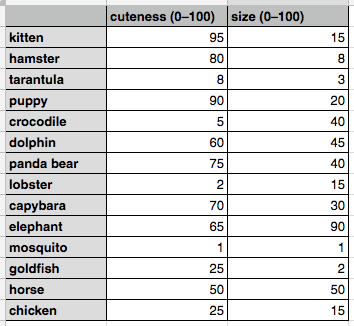
\includegraphics[width=0.6\textwidth]{animal-table.png}
  \caption{This is an example image.}
  \label{fig:example}
\end{figure}

Regardons ce que ça donne en tant qu'espace de vecteurs 2D. 

\begin{figure}[h]
  \centering
  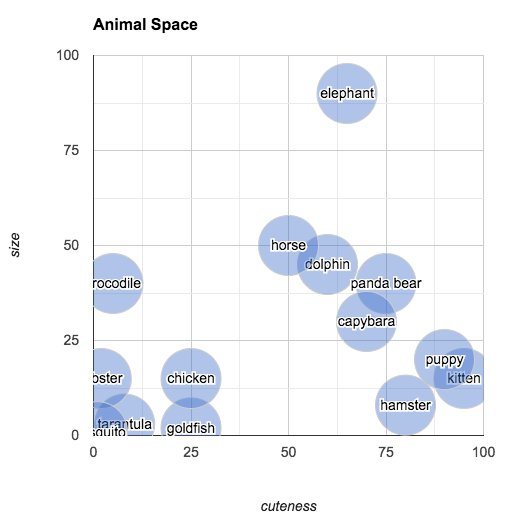
\includegraphics[width=0.6\textwidth]{animal-space.png}
  \caption{This is an example image.}
  \label{fig:example}
\end{figure}

On a associé un objet mathématique (un vecteur 2D) à chaque animal de notre table, certes d'une façon
assez arbitraire, mais pourtant intuitive. Le plus important : on peut maintenant raisonner sur les animaux en 
utilisant les notions de l'algèbre linaire. Par exemple, avec la distance euclidienne, on peut facilement 
vérifier que le cheval et le dauphin sont quasiment les mêmes, quant à nos deux caractéristiques 
(assez mignons et grands). Pareil pour le chiot et le chatons (petits et très mignons), ou bien la 
tarantule et le moustique (très petits et pas du tout mignons). On peut aussi faire des opérations sur 
les vecteurs. Prenons la différence entre le chaton et la poule et ajoutons-la à la tarantule. 

\begin{figure}[h]
  \centering
  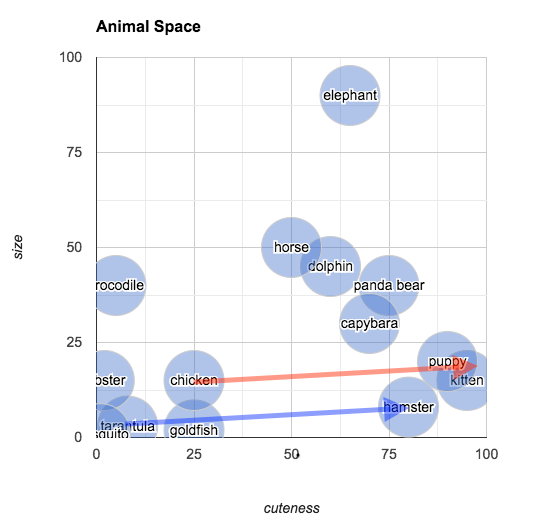
\includegraphics[width=0.6\textwidth]{animal-space-dif.png}
  \caption{This is an example image.}
  \label{fig:example}
\end{figure}

On observe que la pointe du vecteur bleu est le plus près du vecteur qui représent le hamster.
Mathématiquement, cela s'écrirait :

\begin{align*}
  \vec{c} - \vec{p} + \vec{t} \approx \vec{h} 
\end{align*}

Et en français : 

\begin{center}
  Les tarentules sont aux hamsters ce que les poules sont aux chatons. 
\end{center}

C'est-à-dire un animal un peu plus petit et beaucoup moins mignon, ce qui est assez 
correcte. 

Qu'est-ce qui vient de se passer ? On a fait du word embedding sur les 
mots d'animaux, ce qui nous a permis d'analyser leur sémantique par la suite : 
on commence en associant un vecteur à chaque mot en fonction de la mignonnerie et la 
taille de l'animal, on regarde la relation mathématique entre deux mots
(la poule et le chaton), et on utilise cette information pour déduire une \textbf{rélation sémantique} entre deux mots différents
(la tarantule et le hamster). Incroyablement simple et puissant en même temps.

\section*{Sémantique distributionnelle}
Dans les applications réelles des word embeddings, le principe reste le même, mais le processus devient plus 
compliqué. Les mots à l'entrée vont être beaucoup plus nombreux - on peut imaginer un ensemble 
des centaines de milliers de mots. Ensuite, comment fait-on pour associer un vecteur à chacun
de ces mots ? Dans l'exemple précédent, on a attribué des valeur arbitraires à chaque mot 
manuellement, ce qui ne sera plus possible à cause de leur quantité. Heureusement qu'il y a la 
hypothèse distributionnelle. 

\begin{hyp}[hypothèse distributionnelle]
  La sémantique d'un mot est déterminée par son contexte - les mots qui l'entourent dans 
  le texte. 
\end{hyp}

Cette hypothèse dûe à J. R. Firth nous dit que ce qui détermine le sémantique d'un mot 
sont les mots qui se trouvent à ses côtés dans la phrase. Prenons les mots 
beau, froid et chaud et regardons des exemples de 
phrases qui utilisent ces mots : 

\begin{center}
  Il a fait \underline{bien} \textbf{froid} \underline{hier}. \\
  Par contre, il va faire \underline{hyper} \textbf{chaud} \underline{aujourd'hui}. \\
  Il fera \underline{très} \textbf{beau} \underline{demain}! \\
  Est-ce qu'il va faire \underline{très} \textbf{froid} \underline{mardi} ?
\end{center}

Il s'agit des phrases tout à fait naturelles, et on peut déjà observer que les trois mots 
ont une tendance à se trouver entre un adverbe (bien, hyper, très) et un mot indiquant 
un jour (hier, aujourd'hui, demain, mardi). Par la hypothèse distributionnelle, ces trois mots 
devraient avoir une sémantique similaire, car ils ont le même 
contexte. Ceci est tout à fait vrai, tous les trois mots sont utilisés pour décrire le temps. 
Une telle sémantique s'appelle alors comme la hypothèse - distributionnelle. 

Cette approche nous permettra d'assiocer des vecteurs aux mots d'un corpus de taille 
arbitraire, et en plus automatiquement. Regardons sur un exemple :
\begin{center}
  It was the best of times, it was the worst of times.                                                                                                                                                                                                                                                                                                                                                                                                                                                                                                                                                                                                                                                                                                                                                                                                                                                                                                                                                                                                                                                                                                                                                                                                                                                                                                                                                                                                                                                                                                                                                                                                                                                                                                                                                                                                                                                                                                                                                                                                                                                                                                                                                                                                                                                                                                                                                                                                                                                                                                                                                                                                                                                                                                                                                                                                                                                                                                                                                                                                                                                                                                                                                                                                                                                                                                                                                                                                                                                                                                                                                                                                                                                                                                                                                                                                                                                                                                                                                                                                                                                                                                                                                                                                                                                                                                                                                                                                                                                                                                                                                                                                                                                                                                                                                                                                                                                                                                                                                                                                                                                                                                                                                                                                                                                                                                                                                                                                                                                                                                                                                                                                                                                                                                                                                                                                                                                                                                                                                                                                                                                                                                                                                                                                                                                                                                                                                                                                                                                                                                                                                                                                                                                                                                                                                                                                                                                                                                                                                                                                                                                                                                                                                                                                                                                                                                                                                                                                                                                                                                                                                                                                                                                                                                                                                                                                                                                                                                                                                                                                                                                                                                                                                                                                                                                                                                                                                                                                                                                                                                                                                                                                
\end{center}
Comme le contexte, on considérera juste le voisin gauche et le voisin droite. La 
première ligne de la table suivante contient tous les contextes possibles (nb : même si 
"it was the" a deux occurrences dans notre phrase, le contexte correspondant "it \textunderscore \ the" 
ne se trouve qu'une fois dans la table). La première colonne contient tous les mots sans répétition.
Finalement, pour chaque mot, les valeur dans sa ligne indique combien de fois il se trouve dans le contexte
spécifié.  

\begin{table}[h]
    \resizebox{1.2\textwidth}{!}{%
    \begin{tabular}{|c|*{10}{c|}}
        \hline
        g & 
        DÉBUT \textunderscore \ was & 
        it \textunderscore \ the & 
        was \textunderscore \ best & 
        the \textunderscore \ of & 
        best \textunderscore \ times & 
        of \textunderscore \ it & 
        times \textunderscore \ was & 
        was \textunderscore \ worst & 
        worst \textunderscore \ times & 
        of \textunderscore \ FIN \\
        \hline
        it & 1 & 0 & 0 & 0 & 0 & 0 & 1 & 0 & 0 & 0 \\ 
        \hline
        was & 0 & 2 & 0 & 0 & 0 & 0 & 0 & 0 & 0 & 0 \\
        \hline
        the & 0 & 0 & 1 & 0 & 0 & 0 & 0 & 1 & 0 & 0 \\
        \hline 
        best & 0 & 0 & 0 & 1 & 0 & 0 & 0 & 0 & 0 & 0 \\
        \hline 
        of & 0 & 0 & 0 & 0 & 1 & 0 & 0 & 0 & 1 & 0 \\
        \hline 
        times & 0 & 0 & 0 & 1 & 0 & 0 & 0 & 0 & 0 & 1 \\
        \hline 
        worst & 0 & 0 & 0 & 1 & 0 & 0 & 0 & 0 & 0 & 0 \\
        \hline  
    \end{tabular}%
    }
    \caption{Exemple de contexte} 
    \label{tab:example} 
\end{table}

On observe que les vecteurs pour les mots \textit{best} et \textit{worst} sont les mêmes :
$[0,0,0,1,0,0,0,0,0,0]$. La distance euclidienne entre les deux est donc zéro, et par la 
hypothèse distributionnelle, ces deux mots devraient avoir la même signification. Ce n'est pas 
tout à fait le cas, car \textit{best} et \textit{worst} sont des antonymes, pas des synonymes. 
Pourtant, leurs sémantiques sont très proches, et on a réussi à le reconnaître. 

Dans l'exemple précédent, notre corpus (l'entrée textuelle) consistait en une phrase, ce qui 
nous a donné 10 contextes : 10 positions possible pour un mot.  
En réalité, on est emmené à utiliser des corpus beaucoup plus grands, où on aurait donc des 
milliers ou mêmes des millions de contextes possibles - des vecteurs à des milliers ou des 
millions de dimensions. On se doute que ce ne serait pas très 
pratique. Grâce à des techniques de réduction de dimensionalité, on peut transformer des vecteurs 
énormes en vecteurs de taille plus raisonnable : environ 100-300, sans perdre trop 
d'information. Je laisse les détails de cette 
transformation de côté, peut-être si j'ai le temps à la fin.  

\section*{Démonstration}
Il existe de nombreuses collections de vecteurs déjà prêtes qu'on 
peut télécharger et utiliser dans nos projets. Dans l'exemple suivant, 
on utilisera une collection de 514 000 vecteurs de mot en anglais à 300 dimensions. 
Ca fait beaucoup de vecteurs. 

La démonstration suivante est elle aussi fortement inspirée de 
\textit{Understanding word vectors} de Allison Parrish, comme je ne suis pas 
très original et surtout je n'ai pas le temps de développer un exemple intéressant 
moi-même. Pour cela, il faudrait vraiment plonger dans le sujet, et ce n'est pas 
possible, sachant qu'on est à la fin du semeste :)

Je vais utiliser l'un de mes livres préféré comme le corpus. Il s'agit de 
Joyland, écrit par Stephen King. Pour vous mettre un peu dans l'ambiance, 
Joyland parle d'un jeune homme du nom Devin Jones. Devin a 21 ans, il fait 
des études d'anglais, il rêve de devenir écrivant mais sinon il ne sait pas 
quoi faire de sa vie. Sa copine vient de le larguer, et donc au lieu de 
passer les vacances d'été avec elle, il les passe à travailler dans un parc 
d'attraction. Ici il trouve des amis, un boulot qui le plaît. Un peu plus tard, 
il fait enfin la connaissance de la jolie femme blonde qui habite dans l'une des maisons 
qui bordent la plage que Devin traverse pour se rendre au parc. Il y a aussi 
un mystère à résoudre (c'est du Stephen King) : une suite de meurtres de jeunes 
filles, toutes dans des parcs d'attraction, incluant celui où Devin passe son été. 
Tout ça dans une vibe des années 70 en Caroline du Nord. 

On va utiliser SpaCy pour traiter le corpus et pour pouvoir jouer avec les 
vecteurs de mot. Voici le code : 

\begin{figure}[h]
  \centering
  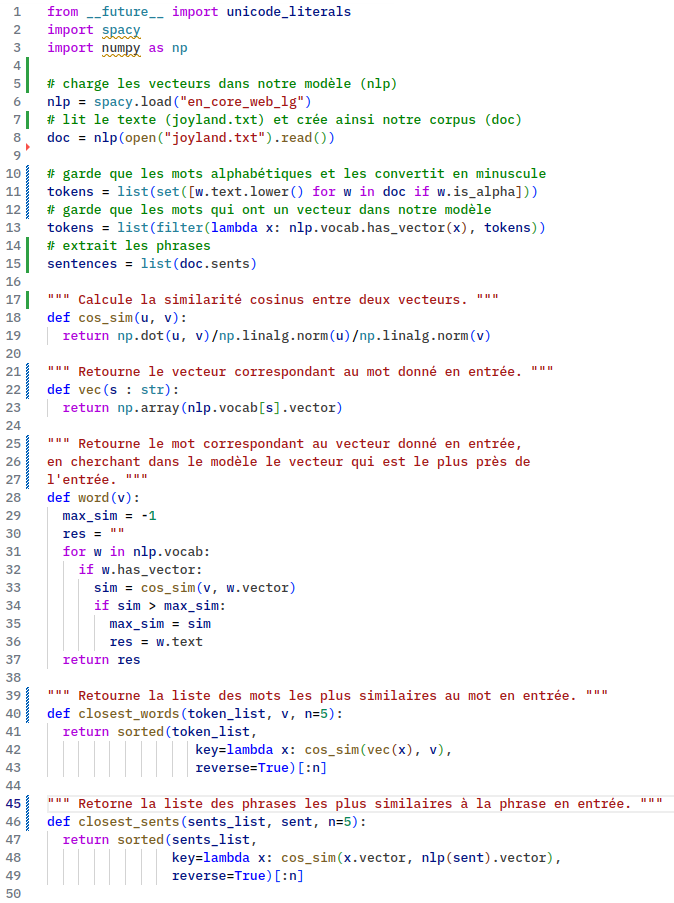
\includegraphics[width=1\textwidth]{code1.png}
  \caption{This is an example image.}
  \label{fig:example}
\end{figure}


\chapter{Deep Learning pour le TALN}
\chapter{Conclusion}

\bibliographystyle{unsrt}
\bibliography{bibliographie}

\end{document}
